% chapters/ch8_exp_dynamic_control.tex --- 5.3 動的制御の実機検証実験
\section{動的制御の実機検証実験}
\label{sec:exp_dynamic_control}

\subsection{実験の目的}

本実験では，動的制御の最小構成として\SI{100}{\milli\second}と\SI{500}{\milli\second}の切替を実装し，固定\SI{100}{\milli\second}および固定\SI{500}{\milli\second}と比較する．平均電力が両固定条件の中間に位置し，受信率も中間的になることを確認し，動的制御が正常に機能していることを検証することを目的とする．

\subsection{実験条件と方法}

評価指標として，省電力指標$q_{\mathrm{event}}$および受信品質指標であるTLと$P_{\mathrm{out}}(\tau)$を用いる．本実験ではtrial長とイベント数$N_{\mathrm{event}}$を固定しているため，$q_{\mathrm{event}}$は平均電力$\overline{P}$と単調対応する．したがって，図表では視認性の高い$\overline{P}$を主に併記し，省電力の解釈は一次KPIである$q_{\mathrm{event}}$と同じ結論になる．

\subsubsection{固定間隔の基準特性}

固定間隔における$q_{\mathrm{event}}$と受信品質を基準として整理する．特に，\SI{100}{\milli\second}から\SI{500}{\milli\second}への変更により電力が低下する一方で，受信率や遅延分布が変化するため，制約$\epsilon$に対する可行性が境界条件として現れる．

\tabref{tab:power_table_example}に，\SI{100}{\milli\second}から\SI{2000}{\milli\second}までの固定間隔における平均電力の一例を示す．表中の各行は固定間隔条件，各列はアドバタイジング間隔，平均電力，および試行数とsleep設定を表す．

\begin{table}[tb]
  \centering
  \caption{固定間隔の平均電力}
  \label{tab:power_table_example}
  \begin{tabular}{lll}
    \toprule
    アドバタイジング間隔 [ms] & 平均電力 [mW] & 備考 \\
    \midrule
    100  & 198.56 & n=10 sleep ON \\
    500  & 180.80 & n=9 sleep ON \\
    1000 & 178.62 & n=9 sleep ON \\
    2000 & 177.47 & n=9 sleep ON \\
    \bottomrule
  \end{tabular}
\end{table}

\tabref{tab:power_table_example}の例では，\SI{100}{\milli\second}から\SI{500}{\milli\second}への変更で平均電力が大きく低下する．ただし，\SI{500}{\milli\second}以上では改善幅が小さくなる．この傾向は，動的制御において短間隔の滞在時間を抑制する設計が有効であることを示唆する．

\subsubsection{動的制御の確認}

動的制御の確認としては，平均電力が両固定条件の中間に位置し，かつログ上でinterval切替が発生することを確認すれば十分である．以降では，TLと$P_{\mathrm{out}}(\tau)$を用いて，QoS制約下での省電力効果を定量評価する．

\subsubsection{実測のQoS指標}

本実験では，受信品質をPDRだけでなく，遅延分布と期限超過率$P_{\mathrm{out}}(\tau)$で評価する．特に，非理想スキャン環境では平均受信率が同程度でも，遅延の裾が悪化する場合があるため，$P_{\mathrm{out}}(\tau)$が重要となる．

\subsection{実験結果}

\tabref{tab:d2_summary}に，scan90における実測例を示す．本表は，S1とS4の2条件について，固定\SI{100}{\milli\second}，固定\SI{500}{\milli\second}，および方策の2値切替の比較をまとめたものである．ここでは初期試行と追加試行を統合し，各条件n=6として集計した．

\begin{table}[tb]
  \centering
  \caption{scan90における動的制御の実測例}
  \label{tab:d2_summary}
  {\scriptsize
  \setlength{\tabcolsep}{3pt}
  \begin{tabular}{lrrrrrr}
    \toprule
    条件 & $P_{\mathrm{out}}(1\,\mathrm{s})$ & $TL_{\mathrm{mean}}$[s] & PDR\_unique & P[mW] & $q_{\mathrm{event}}$ & share100 \\
    \midrule
    S1-100   & 0.075$\pm$0.027 & 3.76$\pm$1.46 & 0.789$\pm$0.016 & 204.1$\pm$1.4 & 561.1$\pm$3.8 & 1.000$\pm$0.000 \\
    S1-500   & 0.142$\pm$0.049 & 5.29$\pm$0.02 & 0.816$\pm$0.018 & 184.7$\pm$1.5 & 502.6$\pm$4.1 & 0.000$\pm$0.000 \\
    S1-policy & 0.125$\pm$0.027 & 5.24$\pm$0.05 & 0.803$\pm$0.022 & 191.5$\pm$1.9 & 523.8$\pm$5.3 & 0.331$\pm$0.004 \\
    \midrule
    S4-100   & 0.053$\pm$0.010 & 1.25$\pm$0.01 & 0.792$\pm$0.009 & 204.4$\pm$2.1 & 274.2$\pm$2.8 & 0.998$\pm$0.002 \\
    S4-500   & 0.146$\pm$0.031 & 2.48$\pm$1.11 & 0.817$\pm$0.020 & 184.5$\pm$1.5 & 245.0$\pm$2.0 & 0.000$\pm$0.000 \\
    S4-policy & 0.069$\pm$0.029 & 1.58$\pm$0.50 & 0.793$\pm$0.021 & 196.6$\pm$1.6 & 262.8$\pm$2.1 & 0.595$\pm$0.008 \\
    \bottomrule
  \end{tabular}
  }
\end{table}

\figref{fig:d2b_power_vs_pout}に，平均電力と$P_{\mathrm{out}}(1\mathrm{s})$の関係を示す．図中の横軸は$P_{\mathrm{out}}(1\mathrm{s})$，縦軸は平均電力であり，各点は固定間隔およびpolicy条件を表す．share100は図中に注記する．

\begin{figure}[tb]
  \centering
  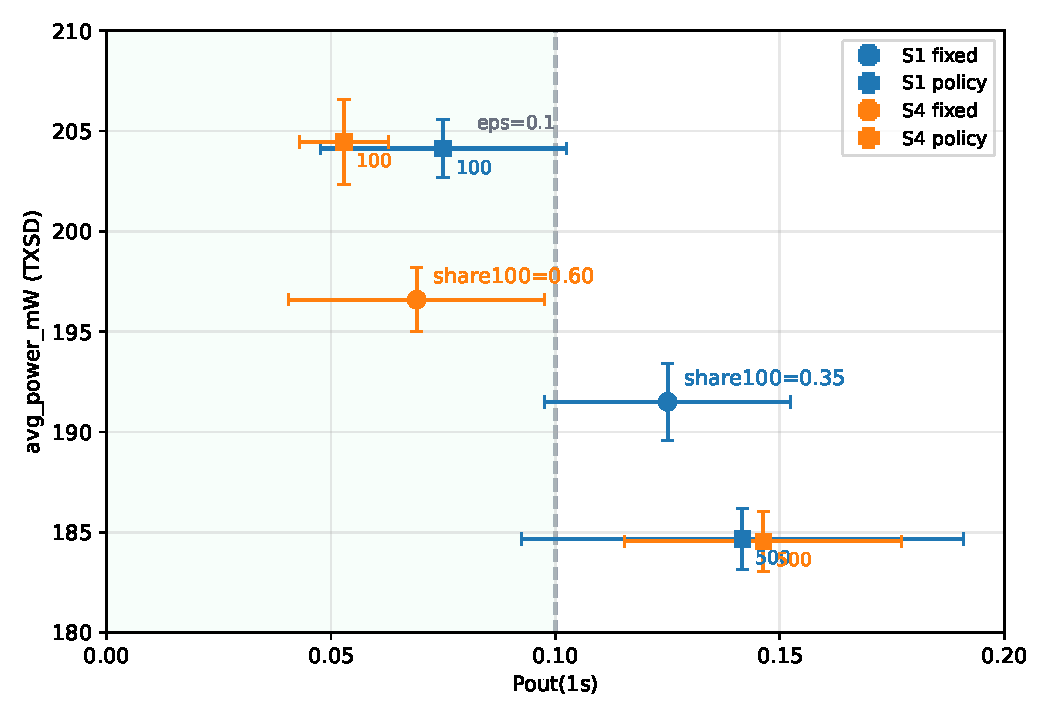
\includegraphics[width=0.90\linewidth]{figures/d2b_power_vs_pout}
  \caption{平均電力と$P_{\mathrm{out}}(1\mathrm{s})$の関係}
  \label{fig:d2b_power_vs_pout}
\end{figure}

\subsection{考察}

\tabref{tab:d2_summary}および\figref{fig:d2b_power_vs_pout}より，方策の2値切替は固定\SI{100}{\milli\second}より低電力であり，固定\SI{500}{\milli\second}より低い期限超過率を示す運用点になり得る．さらに，遷移が多い側であるS4ほどshare100が増加しており，「必要時のみ\SI{100}{\milli\second}を選択し，それ以外は\SI{500}{\milli\second}を選択する」挙動が定量で確認できる．

また，平均電力は固定\SI{100}{\milli\second}と固定\SI{500}{\milli\second}の滞在比率であるshare100による線形混合で概ね説明できるため，方策の省電力効果はinterval滞在比率に支配されることが示唆される．これにより，スリープ実装の詳細に依存する議論から分離し，制御則の議論へ接続しやすくなる．

\clearpage
